\documentclass [a4paper, 11pt] {article}

%document configuration
\newcommand{\courseName}{Machine Learning in Graphics \& Vision}
\newcommand{\termYear}{Summer Term 2020}
\newcommand{\homeworkNum}{5}
\newcommand{\studentOne}{Driton Goxhufi}
\newcommand{\studentTwo} {Damir Ravlija}
\newcommand{\matrikelNrStOne}{4233242}
\newcommand{\matrikelNrStTwo}{5503184}
\newcommand{\mailStOne}{driton.goxhufi@student.uni-tuebingen.de}
\newcommand{\mailStTwo}{damir.ravlija@student.uni-tuebingen.de}

%packages
\usepackage [english] {babel}
\usepackage [T1] {fontenc}
\usepackage [utf8] {inputenc}
\usepackage {graphicx}
\usepackage {subcaption}
\usepackage {amsmath}
\usepackage {amssymb}
\usepackage {amstext}
\usepackage {amsthm}
\usepackage {listings}
\usepackage {tikz}
\usepackage[
pdftex,
pdfauthor={Goxhufi, Driton; Ravlija, Damir},
pdftitle={MLGV - Exercise \homeworkNum Submission},
pdfsubject={Machine Learning in Graphics \& Vision Homework}
]{hyperref}

\usepackage[a4paper,lmargin={2cm},rmargin={2cm},tmargin={3.5cm},bmargin = {2.5cm},headheight = {4cm}]{geometry}

\usepackage[shortlabels]{enumitem}
\usepackage{lastpage}
\usepackage{fancyhdr}

\usepackage{lipsum}
\usepackage{ifthen}

\pagestyle{fancy}



%other config
\renewcommand{\v}[1]{\boldsymbol{#1}}
\newcommand{\mat}[1]{\boldsymbol{#1}}
\newcommand{\m}[1]{\begin{pmatrix}#1\end{pmatrix}}
\newcommand{\tr}[2]{{}^{#1}T_{#2}}
\graphicspath{{./template/out/}}

\lhead{\begin{tabular}{l}
		\courseName\\
		\termYear \\
		Exercise \homeworkNum
\end{tabular}}
\rhead{\begin{tabular}{lr}
		\studentOne & \matrikelNrStOne \\
		\studentTwo & \matrikelNrStTwo \\
\end{tabular}}

\begin{document}
	
\title{\vspace{-1.5cm}\textbf{Exercise \homeworkNum} \\ 
	\courseName}
\author{\begin{tabular}{lcr}
		\studentOne & \matrikelNrStOne & \href{mailto:\mailStOne}{\mailStOne} \\
		\studentTwo & \matrikelNrStTwo & \href{mailto:\mailStTwo}{\mailStTwo} 
\end{tabular}}	
\date{}
\maketitle


\section*{5.1}
\begin{enumerate}
\item[a)]
Visualization of the first 5 principal components:\\
\begin{figure}[!h]
	\centering
	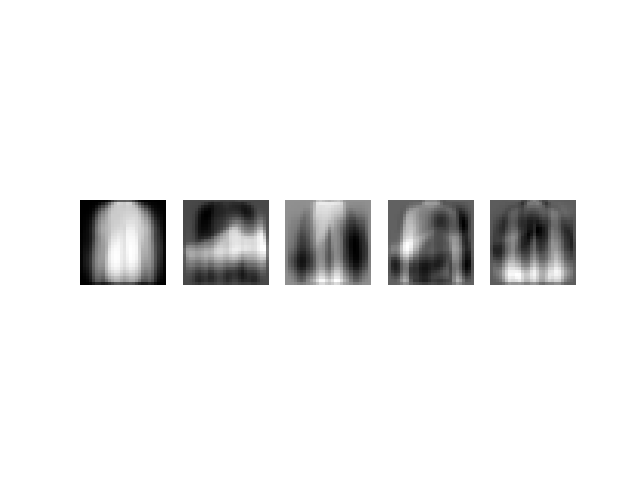
\includegraphics[width=0.8\textwidth]{template/out/pca/pc.png}
	\caption{ 5.1a, output of $compute\_pca(x)$, first 5 principal components.}
\end{figure}

\newpage
\item[(b)]
\begin{figure}[!h]
	\centering
	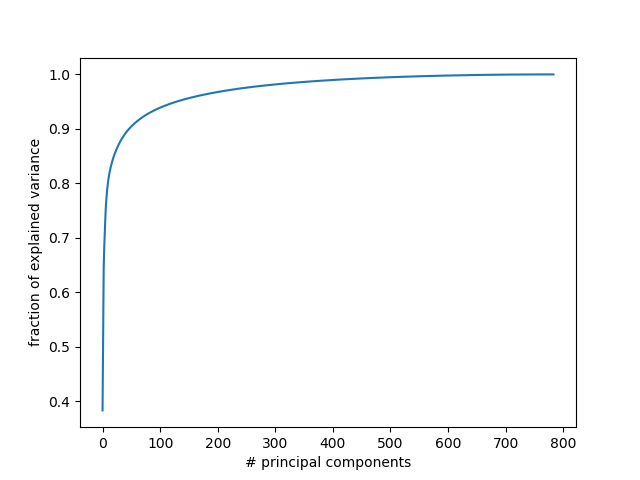
\includegraphics[width=0.8\textwidth]{template/out/pca/cum_dist.png}
	\caption{ 5.1b, the percentage of explained variance over the number of principal components.}
\end{figure}
\begin{lstlisting}
	Entries to achieve 50%: 1
	Entries to achieve 90%: 47
	Entries to achieve 95%: 129
	Entries to achieve 99%: 404
\end{lstlisting}

\newpage
\item[(c)]
Reconstruction:\\
\begin{figure}[!h]
	\centering
	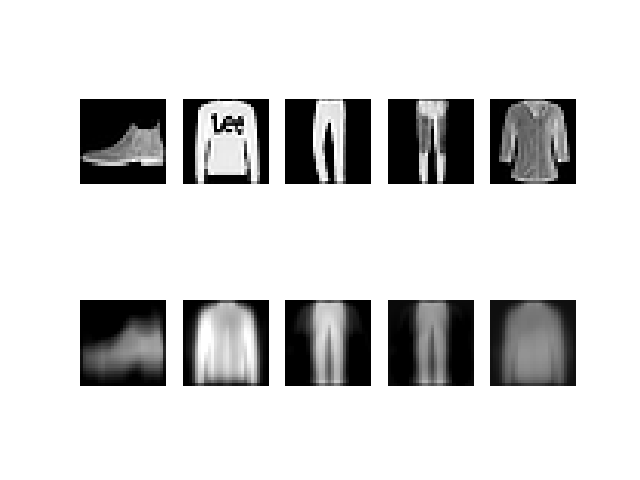
\includegraphics[width=0.8\textwidth]{template/out/pca/recon.png}
	\caption{ 5.1c, reconstruction after compression with PCA.}
\end{figure}

\begin{lstlisting}
	Mean Squared Error:  0.035497293
	Compression Ratio:  156.8
\end{lstlisting}

\newpage
\item[(d)]
Sampling from a gaussian distribution:\\
\begin{figure}[!h]
	\centering
	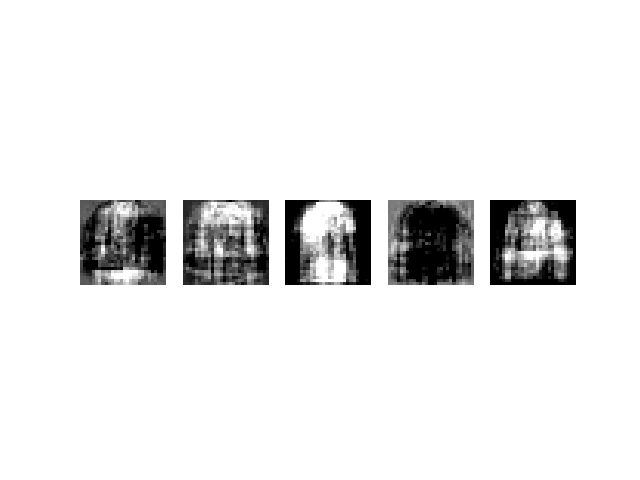
\includegraphics[width=0.8\textwidth]{pca/samples.png}
	\caption{ 5.1d, Synthetic generated samples from a Gaussian distributed model with 5 principle components.}
\end{figure}

\textbf{Do they look realistic?}\\
There are some recognizable contours, but they do not realy look realistic.

\newpage
\item[(e)]
By applying PCA only to the Sneaker-subset, we can obtain better results as shown in the following figures:

\begin{figure}[!h]
	\centering
	\begin{subfigure}{.7\textwidth}
		\centering
		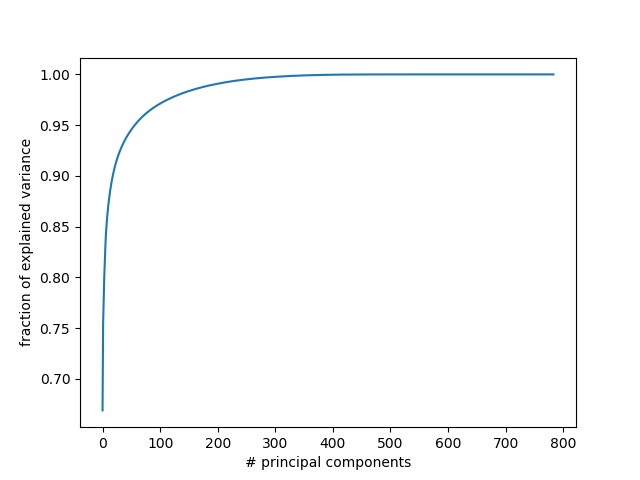
\includegraphics[width=0.8\textwidth]{pca/sneaker/cum_dist.png}
		\caption{cumulative distribution}
		\label{fig:sfig1}
	\end{subfigure}
	\begin{subfigure}{.7\textwidth}
		\centering
		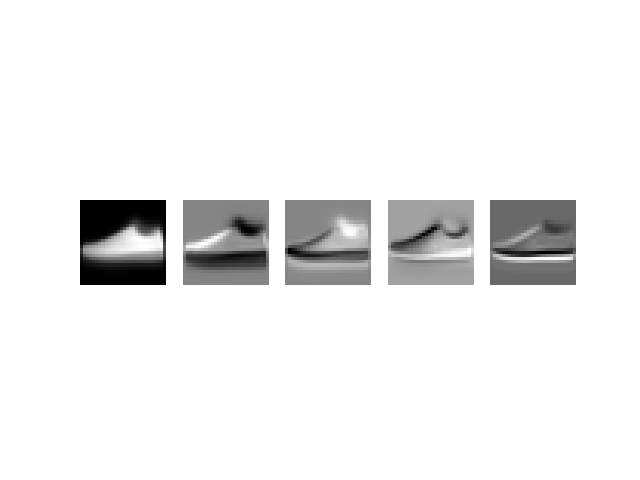
\includegraphics[width=0.8\textwidth]{pca/sneaker/pc.png}
		\caption{principal components}
		\label{fig:sfig2}
	\end{subfigure}
\end{figure}

\begin{figure}[!h]
	\centering
	\begin{subfigure}{.7\textwidth}
		\centering
		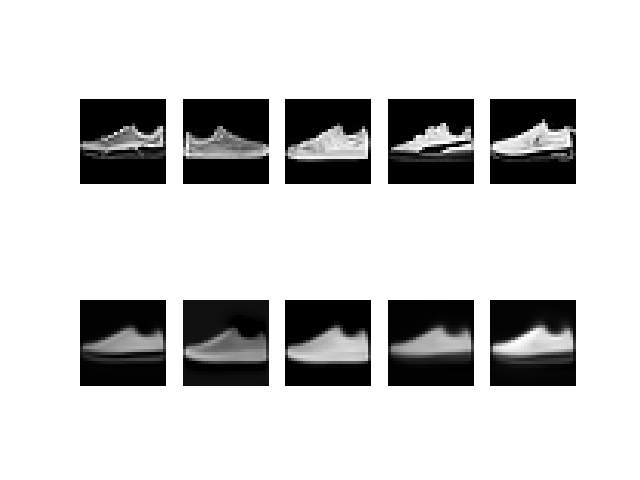
\includegraphics[width=0.8\textwidth]{pca/sneaker/recon.png}
		\caption{reconstruction}
		\label{fig:sfig3}
	\end{subfigure}
	\begin{subfigure}{.7\textwidth}
		\centering
		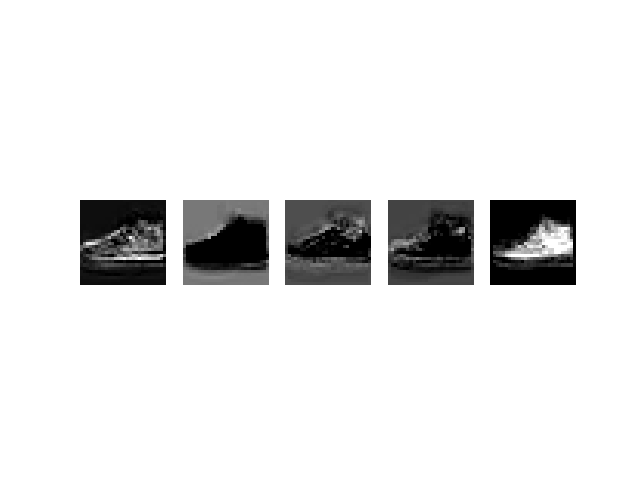
\includegraphics[width=0.8\textwidth]{pca/sneaker/samples.png}
		\caption{synthetic samples}
		\label{fig:sfig4}
	\end{subfigure}
	\caption{ 5.1e, results after applying PCA only to the Sneaker-subset. As we obviously can recognize, the reconstruciton results and the synthetic generation of samples are better than in the tasks before.}
\end{figure}

The other outputs like needed principal components to achieve proper variance of the data decreased and the mean squared error is lower too:
\begin{lstlisting}
	Entries to achieve 50%: 0
	Entries to achieve 90%: 18
	Entries to achieve 95%: 56
	Entries to achieve 99%: 193
	Mean Squared Error:  0.015440599
\end{lstlisting}

\end{enumerate}

\end{document}

